\documentclass[a4paper, 12pt]{article}
\usepackage[T2A]{fontenc}
\usepackage[utf8]{inputenc}
\usepackage[english,russian]{babel}
\usepackage{amsmath, amsfonts, amssymb, amsthm, mathtools, misccorr, indentfirst, multirow}
\usepackage{wrapfig}
\usepackage{graphicx}
\usepackage{subfig}
\usepackage{enumitem}
\usepackage{adjustbox}
\usepackage{pgfplots}

\usepackage{geometry}
\geometry{top=20mm}
\geometry{bottom=20mm}
\geometry{left=20mm}
\geometry{right=20mm}
\newcommand{\angstrom}{\textup{\AA}}
\begin{document}
	\begin{titlepage}
		\begin{center}
		МИНИСТЕРСТВО ОБРАЗОВАНИЯ И НАУКИ РОССИЙСКОЙ ФЕДЕРАЦИИ\\
		\footnotesize{Московский физико-технический институт}\\
		\footnotesize{(государственный университет)}\\
		\vfill
		{\LARGE
		\textbf{Волоконный лазер}\\
		}
		\vspace{1cm}
		Лабораторная работа по курсу\\
		фотоника
		\vfill
		\begin{flushright}
			Выполнили: студенты 654гр.\\
			Нехаев А.С.\\
			Суманова Е.Д.\\
			Тихонов С.С.
		\end{flushright}
		\vfill
		г. Долгопрудный\\
		\the\year\:год
		\end{center}
	\end{titlepage}
	\newpage
	\pagenumbering{arabic}
	\tableofcontents
	\newpage
	\section{Цели и задачи исследования}
	\begin{enumerate}
		\item Изучить генерацию в волоконном лазере в режиме свободной генерации и физические основы появления релаксационных колебаний.
		\item Изучить методы создания инверсии, управления режимами генерации и формирования модовой структуры излучения в лазере.
		\item Определить влияние параметров генерации на частоту и затухание релаксационных колебаний.
		\item Решить задачи.
	\end{enumerate}
	\newpage
	\section{Теоретическая часть}
	\subsection{Введение}
	Волоконные лазеры являются выдающимся достижением квантовой электроники с момента созданя первого лазера на кристалле рубина в 1960 г.\par
	Поскольку в кварцевом волокне энергия фононов составляет 400-1100 см$^{-1}$, то в качестве активных ионов могут быть использованы только те, у которых энергетический зазор между уровнями с оптическими переходами превышает эту величину, поскольку иначе безизлучательная релаксация приведет к ухудшению люминесценции. Наиболее часто используемые активные ионы это:
	\begin{itemize}[noitemsep]
		\item неодим Nd$^{3+}$ (0.92 -- 0.94 мкм, 1.05 -- 1.1 мкм, 1.34 мкм),
		\item гольмий Ho$^{3+}$ (1.9 -- 2.1 мкм),
		\item эрбий Er$^{3+}$ (1.53 -- 1.6 мкм),
		\item тулий Tm${3+}$ (1.7 -- 1.9 мкм),
		\item иттербий Yb$^{3+}$ (0.98 -- 1.16 мкм).
	\end{itemize}\par
	Преимущества волоконных активных сред по сравнению с объемными активными лазерными средами:
	\begin{itemize}[noitemsep]
		\item низкие оптические потери;
		\item большая длина взаимодействия и малый размер световедущей сердцевины, что обеспечивает эффективную накачку полупроводниковым лазером;
		\item большое отношение площади поверхности волокна к объему, что улучшает теплоотвод;
		\item высокое качество поперечной структуры пучка;
		\item использование внутриволоконных брегговских решеток в качестве распределенных зеркал обеспечивает компактность и стабильность лазера.
	\end{itemize}
	\subsection{Инверсия активной среды как необходимое условие генерации лазера}
	Излучение лазера рождается на переходах между определенными энергетическими уровнями активных центров; их называют \textbf{рабочими уровнями}. Отнесенные к единице объема активной среды заселённости рабочих уровней будем обозначать через $n_1$ (нижний рабочий уровень) и $n_2$ (верхний рабочий уровень). Разность
	\begin{equation}
		N=n_2-(g_1/g_2)n_1
	\end{equation}
	называют плотностью инверсной заселенности рабочих уровней. Здесь $g_1$ и $g_2$ -- кратности вырожденных соответствующих уровней; для простоты будем, как правило, полагать, что $g_1=g_2$.\par
	Если выполняется условие
	\begin{equation}
		N>0
	\end{equation}
	то говорят, что имеет место инверсия активной среды.\par
	Для создания инверсии необходимо перевести активную среду в неравновесное состояние. Обеспечение инверсии активной среды является необходимой предпосылкой для реализации в лазере режима генерации. Коэффициенты усиления $\chi_1$ пространственно-однородной среды описывается выражением
	\begin{equation}
		\chi_1=\sigma N
	\end{equation}
	где $\sigma$ - сечение вынужденных переходов между рабочими уровнями.\par
	Для создания и поддержания инверсии применяют тот или иной способ возбждения (или, как говорят, способ накачки) активной среды. Активная среда лазера представляет собой некий термостат (сердцевина волокна из стекла), в котором имеются активные центры -- квантовые системы, способные в результате возбуждения переходить в состояние с отрицательной температурой, отвечающей инверсной заселенности уровней.\par
	В твердотельных волоконных лазерах активными центрами чаще всего служат ионы с незаполненными внутренними оболочками.\par
	Реальные активные центры обычно имеют богатую систему энергетических уровней. Однако для работы лазера существенную роль играют лишь некоторые из них, в связи с чем при расчетах систему уровней упрощают, рассматривая только необходимые. Чаще всего используют 3-х и 4-х уровневые модели лазера, реже - многоуровневые.
	\subsection{Получение инверсной населенности с помощью когерентной оптической накачки}
	В волоконных лазерах активное волокно имеет сердцевину, легированную ионами редкоземельных металлов, внутреннюю оболочку, образующую с сердцевиной волновод, и внешнюю оболочку, образующую волновод с внутренней оболочкой по которому распространяется излучение накачки, введенное в эту область от полупроводникового лазера. Для излучения накачки волновод является многомодовым, в то же время сердцевина активной области образует одномодовый волновод для генерируемого излучения. Для ввода излучения накачки используется несколько методов:
	\begin{enumerate}
		\item торцевой
		\item набор V-образных канавок, распределенных по боковой поверхности световода;
		\item два световода размещаемых в общей оболочке, один из которых - активный, а в другой вводится излучение накачки, которое в месте их контакта проходит в активную область и осуществляет накачку. Таким образом, осуществляется распределенная накачка активной области.
	\end{enumerate}
	\subsection{Режим работы волоконного лазера – режим свободной генерации}
	Режим свободной генерации фактически означает отсутствие какого-либо специального управления генерацией или какого-либо воздействия на нее извне. В частности, отсутствует какая-либо модуляция (как активная, так и пассивная) добротности резонатора. Свободная генерация может иметь место как в случае импульсной, так и в случае непрерывной накачки. Свободное излучение волоконного лазера представляет собой, как правило, последовательность относительно коротких импульсов или, как принято говорить, пичков. Длительность отдельного пичка равна $10^{-7}-10^{-6}с$ (0.1 - 1 мкс); мощность достигает значений $10^4-10^5$ Вт. Временной интервал между писками составляет примерно 1-10 мкс.
	\begin{figure}[!htb]
		\centering
		\minipage{0.45\textwidth}
		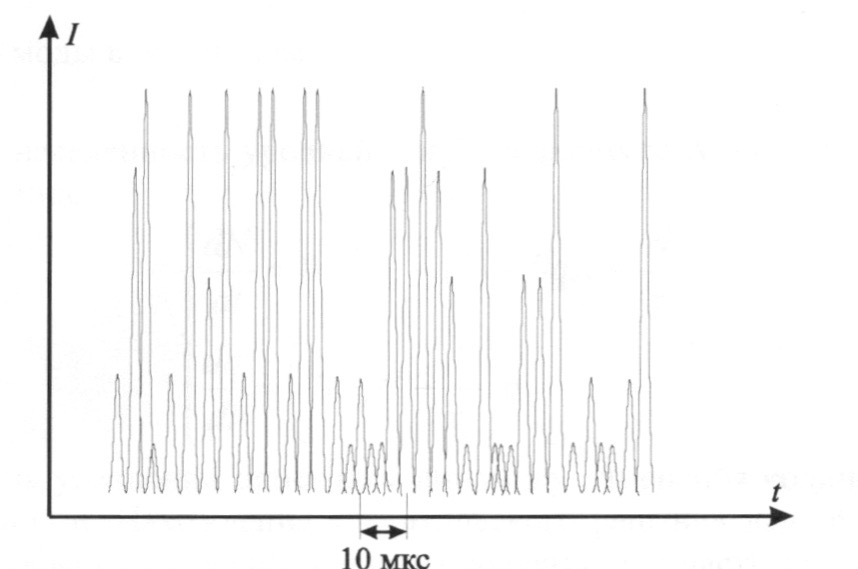
\includegraphics[width=\linewidth]{pic1.jpg}
		\caption{Осциллограмма излучения твердотельного лазера, работающего в режиме свободной генерации}
		\endminipage\hfill
		\minipage{0.45\textwidth}
		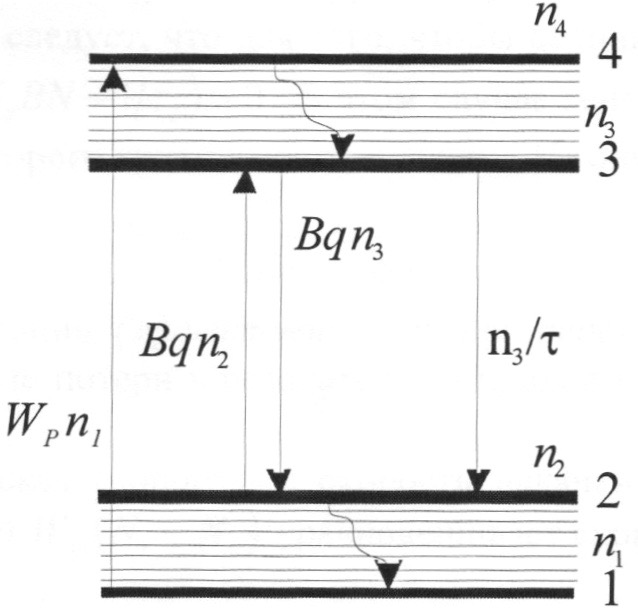
\includegraphics[scale=0.2]{pic2.jpg}
		\caption{Энергетическая схема квази-четырехуровневого лазера}
		\endminipage
	\end{figure}
	\subsection{Динамика генерации лазера в различных режимах работы}
	\subsubsection{Система уравнений, описывающая динамику генерации лазера}
	Считая, что переходы между уровнями 4 и 3 и уровнями 2 и 1 являются быстрыми, можно положить $n_4\approx n_3\approx 0$. В этом случае скоростные уравнения можно записать следующий образом
	\begin{equation}
		\begin{cases}
			\frac{dn_3}{dt}=W_pn_1-Bqn_3-\frac{n_3}{\tau}\\
			\frac{dq}{dt}=V_aBqn_3-\frac{q}{\tau_c}
		\end{cases}
		\label{eq5.1}
	\end{equation}
	\begin{equation*}
		n_1+n_3=N_t
	\end{equation*}
	где:
	\begin{itemize}[noitemsep]
		\item $N_t=8\cdot10^{19}$ ионов/см$^3$ -- плотность ионов иттербия Yb$^{3+}$
		\item $n_1$ -- населенность основного состояния
		\item $n_3$ -- населенность рабочего уровня
		\item $q$ -- полное число фотонов в резонаторе
		\item $W_p$ -- скорость накачки
		\item $\lambda=1.064$ мкм -- длина волны генерации
		\item $\gamma$ -- потери в резонаторе за проход в одном направлении
		\item $V_a=\pi\omega_0^2 l/4$ -- объем моды в активной среде
		\item $B$ -- скорость индуцированных переходов на один фотон в моде
		\item $\omega_0$ -- размер перетяжки моды в резонаторе
		\item $L$ -- длина резонатора
		\item $l$ -- длина активной зоны
		\item $L'=L+\left(n_0-1\right)l$ -- оптическая длина резонатора
		\item $n_0$ -- показатель преломления активной среды
		\item $V=\pi\omega_0^2L'/4$ -- объем моды в резонаторе
		\item $c=2,99792458\cdot 10^{10}$ cм/с -- скорость света
	\end{itemize}
	\par
	Выражения для введенных величин $B$ и $\tau_c$ через известные параметры лазера можно получить следующем виде:
	\begin{equation*}
		B=\frac{\sigma l c}{V_aL'}=\frac{\sigma c}{V}\qquad\tau=\frac{L'}{c\gamma}
	\end{equation*}
	\par
	Вводя инверсную заселенность уровней 3 и 2 по формуле $N=n_3-n_2\approx n_3$ систему уравнений (\ref{eq5.1}) можно переписать в виде:
	\begin{equation}
		\begin{cases}
			\frac{dn_3}{dt}=W_p\left(N_\tau-N\right)-BqN-\frac{N}{\tau}\\
			\frac{dq}{t}=\left(V_aBN-\frac{1}{\tau_c}\right)q
		\end{cases}
		\label{eq526}
	\end{equation}
	Полученная система уравнений описывает динамику изменения количества фотонов в резонаторе и инверсии населенности.\par
	Рассмотрим работу лазера при стационарной накачке (то есть когда скорость накачки $W_p$ не зависит от времени).\par
	Определим пороговое условие генерации лазера.  Предположим, что в момент времени $t=0$ в резонаторе, вследствие спонтанного испускания, присутствует некоторое небольшое число фотонов $q$. При этом из уравнения (\ref{eq526}) следует, что для того, чтобы величина $\frac{dq}{dt}$ была положительной, должно выполняться условие $\left(V_aBN-1/\tau_c\right)$. В этом случае генерация возникнет, если инверсия населенности $N$ достигнет критического значения $N_c$, определяемого выражением
	\begin{equation}
		N_c=\frac{1}{V_aB\tau_c}=\frac{\gamma}{\sigma l}
	\end{equation}
	где:
	\begin{itemize}[noitemsep]
		\item $\sigma$ -- сечение перехода генерации (\textit{эффективное сечение перехода генерации для ионов Yb$^{3+}\ \sigma=2.5\cdot10^{-20}\text{см}^2$})
		\item $\gamma$ -- суммарные потери в резонаторе за проход в одном направлении, определяемые ниже
	\end{itemize}
	\par
	Таким образом, критическая (пороговая) скорость накачки соответствует ситуации, когда полная скорость накачки уровней $W_{cp}\left(N_t-Nc\right)$ уравновешивает скорость $N_c/\tau$ спонтанных переходов с рабочего уровня:
	\begin{equation}
		W_{cp}=\frac{N_c}{(N_t-N_c)\tau}
	\end{equation}
	\par
	Пороговую скорость накачки уровней можно получить
	\begin{equation}
		W_{cp}=\frac{1}{(\tau_cV_aBN_t-1)\tau}
		\label{eq:5.5}
	\end{equation}
	Если $W_p>W_{cp}$, то число фотонов $q$ будет возрастать от начального значения, определяемого спонтанным излучением, и если $W_p$ не зависит от времени, то, в конце концов, достигнет некоторого постоянного значения $q_0$. Это стационарное значение и соответсвующее ему значение инверсии $N_0$ получаются из уравнений (\ref{eq526}), если в них положить $\dot N=\dot q=0$.
	\begin{equation}
		N_0=\frac{1}{V_aB\tau_c}=N_c,\qquad
		q_0=V_a\tau_c\left[W_p\left(N_t-N_c\right)-\frac{N_0}{\tau}\right].
		\label{eq:56}
	\end{equation}
	\par
	Полученные уравнения описывают непрерывный режим работы четырехуровневого лазера. При $W_p=W_{cp}$ имеем $N=N_c$ и $q_0=0$. Заметим, что при накачке ниже пороговой $q=0$, и получаем $N_0=W_p\frac{N_t\tau}{1+W_p\tau}$. Но поскольку обычно выполняется условие $N_0=N_c\ll N_t$, из формулы (\ref{eq:5.5}) находим, что $W_{cp}\tau\ll 1$, то есть $W_p\tau\ll 1$ и $N$ увеличивается с $W_p$ практически линейно. Число фотонов, определяемое в (\ref{eq:56}), можно записать в эквивалентном виде:
	\begin{equation}
		q_0=\left(V_aN_c\right)\left(\tau_c/\tau\right)\left(x-1\right)
	\end{equation}
	где:
	\begin{equation}
		x=W_p/W_{cp}
	\end{equation}
	и где $x$ -- относительное превышение скорости накачки над пороговой. Как для оптической, так и для электрической накачки, модно записать:
	\begin{equation}
		x=P_p/P_{\text{пор}},
	\end{equation}
	где
	\begin{itemize}[noitemsep]
		\item $P_p$ -- мощность электрической накачки (приложенная к лампе или к разряду),
		\item $P_{\text{пор}}$ -- ее пороговое значение.
	\end{itemize}
	Таким образом, если выбрать $P_p/P_{\text{пор}}=1.1$, то количество фотонов в резонаторе будет около $10^{10}$.\par
	Если считать основными потерями в резонаторе -- выход излучения через зеркала, то суммарная мощность излучения, выходящего через оба зеркала:
	\begin{equation}
		P=\frac{q_0\hbar\omega}{\tau_0},
	\end{equation}
	где $\tau_0$ -- время жизни фотонов в резонаторе, определяемое как
	\begin{equation}
		\frac{1}{\tau_0}=-\frac{c}{2L}\ln\left(1-T\right),
	\end{equation}
	где $T$ -- коэффициент пропускания выходного зеркала.
	\subsubsection{Релаксационные колебания в лазере. Работа лазера в нестационарных режимах генерации при ступенчатом включении импульса накачки.}
	Рассмотрим работу лазера при нестационарной накачке. Для данной временной зависимости скорости накачки $W_p(t)$, можно найти временную зависимость q(t) и N(t), если заданы начальные условия.\par
	В случае, когда скорость накачки описывается ступенчатой функцией, будем считать, что скорость накачки имеет следующую временную зависимость: $W_p=0$ при $t<0$ и $W_p(t)=W_p$ (с независящей от времени величиной $W_p$) при $t>0$. При  небольших колебаниях инверсии и количества фотонов около стационарных значений $N_0$ и $q_0$, можно записать
	\begin{equation}
		\begin{cases}
			N(t)=N_0+\delta N\\
			q(t)=q_0+\delta q\\
		\end{cases},
	\end{equation}
	где $\delta N\ll N_0$ и $\delta q\ll q_0$ (так что произведениями типа $\delta N\delta q$ в (\ref{eq526}) можно пренебречь). Тогда из уравнений (\ref{eq526}) получаем систему:
	\begin{equation}
		\begin{cases}
			\delta\dot{N}=-\delta N\left(W_p-\frac{1}{\tau}\right)-B\left(q_0\delta N+N_0\delta q\right)\\
			\delta\dot{q}=Bq_0V_a\delta N
		\end{cases}
		\label{eq:512}
	\end{equation}
	Подстановка нижнего уравнения из (\ref{eq:512}) в верхнее уравнение с учетом $BV_aN-1/\tau_c=0$, дает уравнение колебаний:
	\begin{equation}
		\delta \ddot{q}+\left[W_p+\left(\frac{1}{\tau}\right)+Bq_0\right]\delta\dot{q}+(B^2N_0q_0V_a)\delta q = 0,
	\end{equation}
	Решение которого имеет вид
	\begin{equation*}
		\delta q=\delta q_0\exp(st).
	\end{equation*}
	В этом случае получаем уравнение с параметром $s$:
	\begin{equation*}
		s^2+\left(\frac{2}{t_0}\right)s+\omega^2=0,
	\end{equation*}
	где
	\begin{equation*}
		\omega^2=B^2N_0q_0\qquad\frac{1}{t_0}=\frac{1}{2}\left(W_p+(1/\tau)+Bq_0\right).
	\end{equation*}
	Решение квадратного уравнения будет:
	\begin{equation*}
		s=-1/t_0\pm[(1/t_0)^2-\omega^2]^{1/2}
	\end{equation*}
	где для случая $(1/t_0)<\omega$ вводим $\omega'$ и получаем:
	\begin{equation*}
		\omega'=[\omega^2-(1/t_0)]^{1/2},\qquad s=-1/t_0\pm i\omega'.
	\end{equation*}
	В этом случае решение будет представлять собой затухающее гармоническое колебание:
	\begin{equation}
		\delta q=C\exp(-t/t_0)\sin(\omega't+\varphi)
	\end{equation}
	где константы $C$ и $\varphi$ определяются начальными условиями. Для изменения инверсии в случае $(1/t_0)\ll\omega'$ получаем
	\begin{equation*}
		\delta N=(\omega' C/Bq_0V_a)\exp(-t/t_0)\sin(\omega't+\varphi)
	\end{equation*}
	С учетом (\ref{eq:56}) и считая, что $N_0\ll N_t$, выражения для $t_0$ и $\omega$ можно записать в более простом виде:
	\begin{equation}
		t_0=2\tau/x\qquad\omega=\left(\frac{x-1}{\tau_0\tau}\right)^{1/2},
	\end{equation}
	где $x=W_p/W_{cp}$ --- относительное превышение скорости накачки над пороговой. Таким образом, при ступенчатом включении накачки при генерации лазера происходят затухающие релаксационные колебания количества фотонов в резонаторе и, следовательно, выходной мощности с частотой $\omega'$.\par
	Проведенный анализ режимов работы лазера дает качественную картину динамики генерации лазера при постоянной накачке в режиме непрерывной генерации и в переходном режиме. Численное интегрирование системы уравнений (\ref{eq526}) при расчете параметров генерации лазера показывает следующие зависимости на рисунке \ref{pic:3} развития генерации от времени:
	\begin{figure}[!htb]
		\centering
		\minipage{0.5\textwidth}
		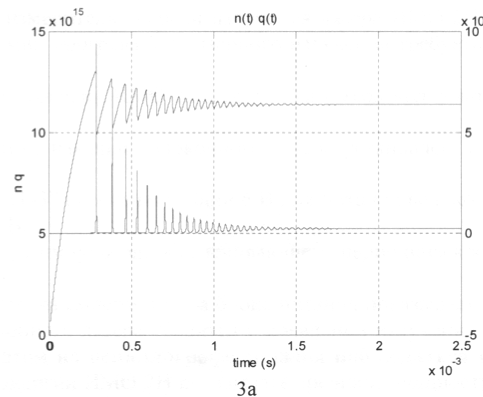
\includegraphics[width=\linewidth]{3a.png}
		\endminipage\hfill
		\minipage{0.5\textwidth}
		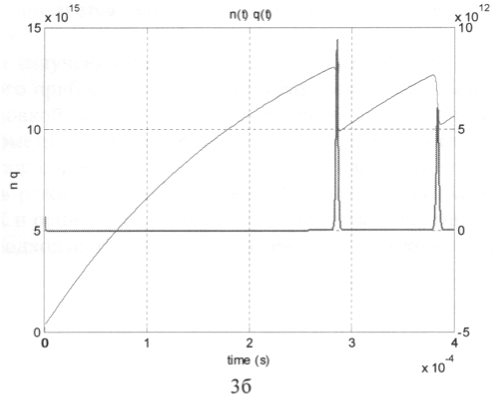
\includegraphics[width=\linewidth]{3b.png}
		\endminipage
		\caption{Зависимость инверсии населенности $n(t)$ и полного числа фотонов в резонаторе $q(t)$ от времени при ступенчатом включении накачки (а и б – показано в разных временных масштабах).}
		\label{pic:3}
	\end{figure}
	\par
	Таким образом, при генерации лазера могут наблюдаться релаксационные колебания мощности генерации (рис.\ref{pic:3}) с частотой, определяемой параметрами лазерной системы. В стационарном режиме генерации инверсия устанавливается на уровне пороговой.
	\newpage
	\section{Практическая часть}
	\begin{enumerate}
		\item Построим график зависимости выходной мощности излучения от мощности накачки
		\begin{table}[h]
			\centering
			\caption{Экспериментальные данные}
			\begin{tabular}{|c|c|c|c|c|}
				\hline
				$I_{\text{накачки}}$, А & Напряжение, В & Показания калориметра, Дж & $W_{\text{выходное}}$, Вт & $W_{\text{накачка}}$, Вт\\
				\hline
				2.1 & 6 & 49 & 1.323 & 12.6\\
 				1.9 & 6 & 46 & 1.242 & 11.4\\
			 	1.8 & 6 & 45 & 1.215 & 10.8\\
 				1.7 & 6 & 43 & 1.161 & 10.2\\
 				1.6 & 6 & 41 & 1.107 & 9.6\\
 				1.5 & 6 & 36 & 0.972 & 9.0\\
			 	1.4 & 6 & 32 & 0.864 & 8.4\\
 				1.3 & 6 & 29 & 0.783 & 7.8\\
 				1.2 & 6 & 25 & 0.675 & 7.2\\
 				1.1 & 6 & 21 & 0.567 & 6.6\\
 				1.0 & 6 & 17 & 0.459  & 6.0\\
 				\hline
			\end{tabular}
		\end{table}
		\begin{figure}[!htb]
			\begin{tikzpicture}
				\begin{axis}[
				xlabel={$W_{\text{накачка}}$, Вт},
				ylabel={$W_{\text{выходное}}$, Вт},
				xmin=2,
				xmax=13,
				ymin=0,
				ymax=1.5,
				ymajorgrids=true,
    			xmajorgrids=true,
    			grid style=dashed,
    			width=\textwidth,
				]
				\addplot[
				color=black,
				mark=square,
				only marks,
				]
				coordinates{
				(6, 0.459)
				(6.6, 0.567)
				(7.2, 0.675)
				(7.8, 0.783)
				(8.4, 0.864)
				(9.0, 0.972)
				(9.6, 1.107)
				(10.2, 1.161)
				(10.8, 1.215)
				(11.4, 1.242)
				(12.6, 1.323)
				};
				\addplot[
				domain=2:13,
				samples=3,
				color=black
				]
				{-0.552857+0.169714*x};
				\end{axis}
			\end{tikzpicture}
			\caption{График зависимости выходной мощности от накачки}
		\end{figure}
		\newpage
		По графику видим, то пороговая мощность накачки равняется примерно $W_{cp}\approx 3.26$ Вт, КПД примерно $\eta\approx 16.97\%$.
		\item Снятие зависимости частоты релаксационных колебаний от превышения над порогом генерации:
		\begin{figure}[h]
			\minipage{0.44\textwidth}
			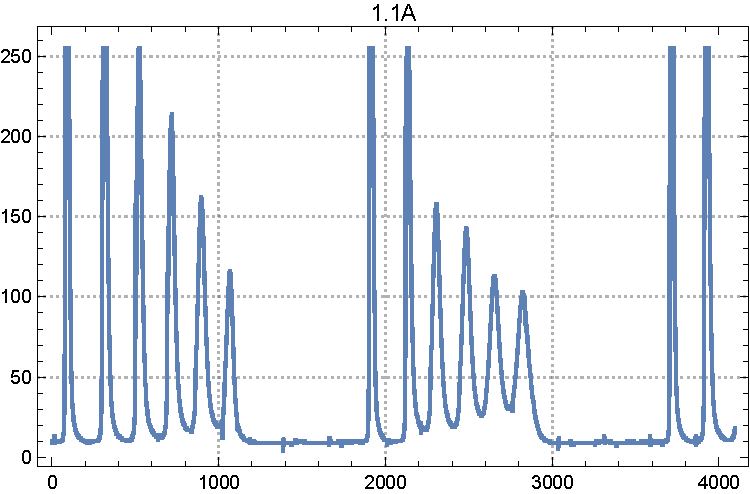
\includegraphics[width=\linewidth]{1.1A.pdf}
			\endminipage\hfill
			\minipage{0.44\textwidth}
			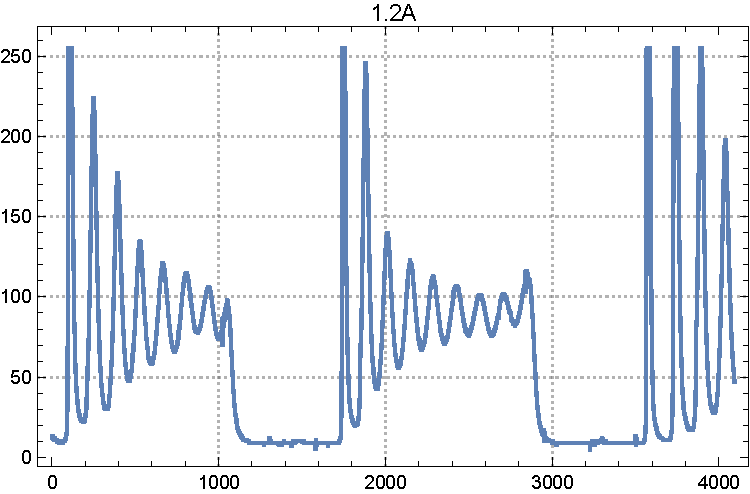
\includegraphics[width=\linewidth]{1.2A.pdf}
			\endminipage\hfill
			\minipage{0.44\textwidth}
			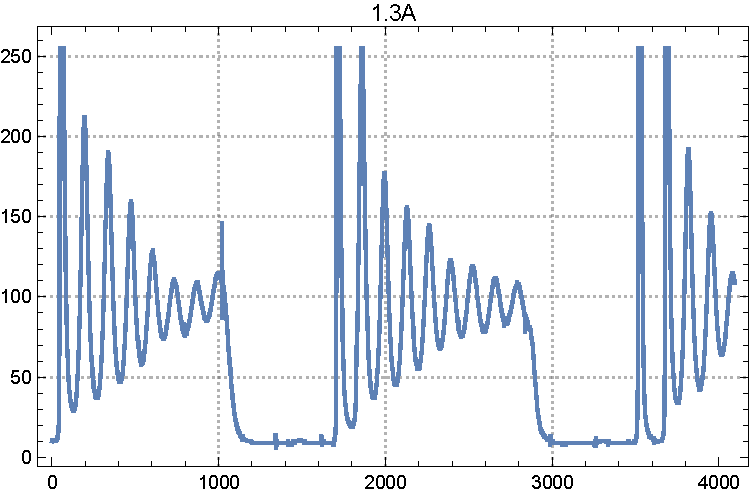
\includegraphics[width=\linewidth]{1.3A.pdf}
			\endminipage\hfill
			\minipage{0.44\textwidth}
			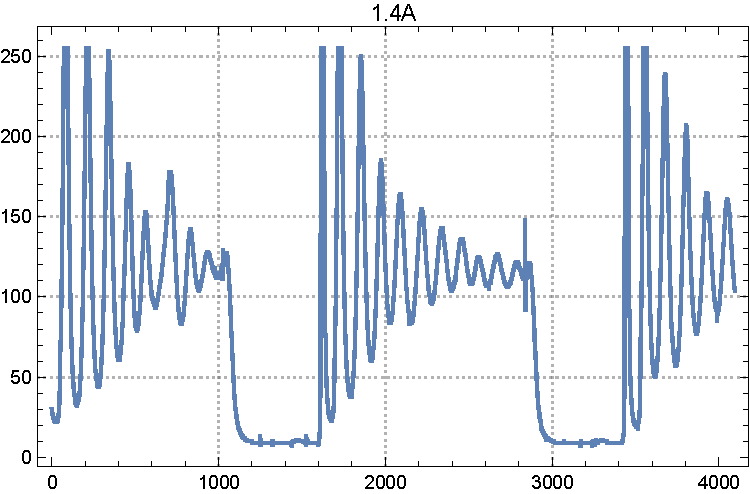
\includegraphics[width=\linewidth]{1.4A.pdf}
			\endminipage\hfill
			\minipage{0.44\textwidth}
			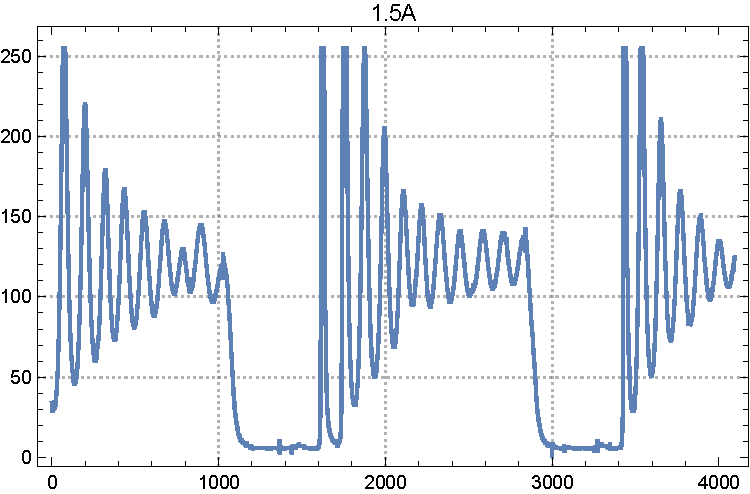
\includegraphics[width=\linewidth]{1.5A.pdf}
			\endminipage\hfill
			\minipage{0.44\textwidth}
			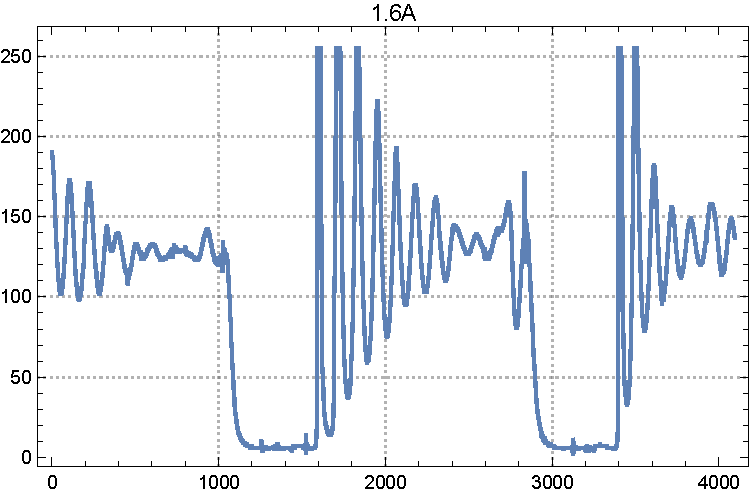
\includegraphics[width=\linewidth]{1.6A.pdf}
			\endminipage\hfill
			\minipage{0.44\textwidth}
			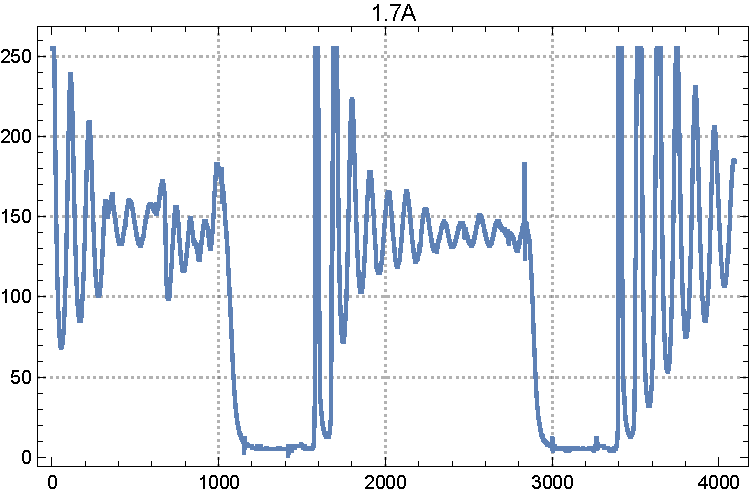
\includegraphics[width=\linewidth]{1.7A.pdf}
			\endminipage\hfill
			\minipage{0.44\textwidth}
			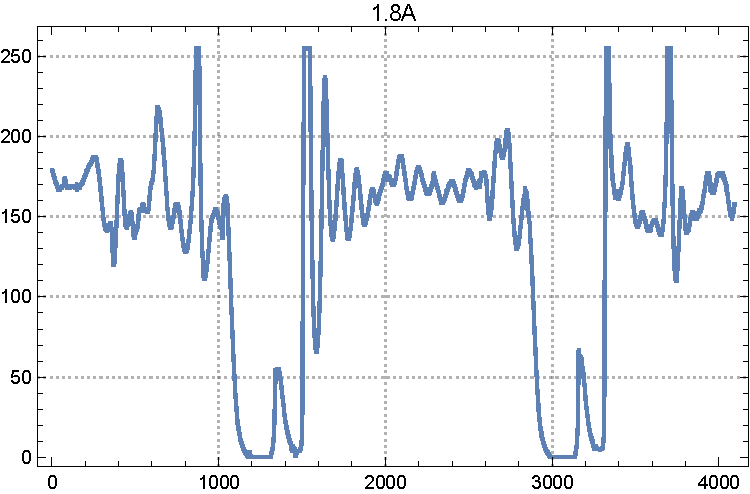
\includegraphics[width=\linewidth]{1.8A.pdf}
			\endminipage
		\end{figure}
		\par
		%Также проведем теоретический расчёт частоты релаксационных колебаний для лазера с параметрами: $L'=10$м, $\gamma=0.12$, $t_0=1.4$ мс, $\tau_c=278$ нс.%
	\end{enumerate}
	\newpage
	\section{Задачи}
	\begin{enumerate}
			\item Рассчитать частоту релаксационных колебаний для волоконного лазера, используемого в работе.
			\begin{equation*}
				\omega=\sqrt{\frac{x-1}{\tau_0\tau}};\quad x=\frac{W_p}{W_{cp}};\quad \frac{1}{\tau_0}=-\frac{c}{2L}\log\left(1-T\right).
			\end{equation*}
			\begin{equation*}
				T=0.8;\quad \tau=1200 \text{ мкс};\quad L=10\text{ см}.
			\end{equation*}
			\begin{equation*}
				\omega=\sqrt{\frac{0.5}{1200\times10^{-6}\times\frac{-20}{3\times10^8}\left(\log0.2\right)^{-1}}}=100294.5\text{ Гц}
			\end{equation*}
			\item Определить время затухания фотонов в резонаторе волоконного лазера.
			\begin{equation*}
				\frac{1}{\tau_0}=-\frac{c}{2L}\log\left(1-T\right)\Rightarrow \tau_0=40\text{ нс}
			\end{equation*}
			\item Определить температуру, при которой работа иттербиевого лазера будет происходить по трехуровневой схеме, если штарковское расщепление уровней рабочего перехода $\sim 500\text{ см}^{-1}$
				\begin{equation*}
					E=\hbar\omega=\hbar c \frac{2\pi}{\lambda}=kT\Rightarrow T=\frac{2\pi\hbar c}{k}=\frac{hc}{\lambda k}
				\end{equation*}
				\begin{equation*}
					W=\frac{1}{\lambda}=\frac{1}{500\text{ см}}\Rightarrow T=\frac{hcW}{k}=720\text{К}
				\end{equation*}
			\item Рассчитать частоту и время затухания релаксационных колебаний для типичного He-Ne, полупроводникового и YAG:Nd$^{3+}$ лазеров.
			\begin{equation*}
				\tau_0=-\frac{2L}{c\cdot\log\left(1-T\right)}
			\end{equation*}
			\begin{equation*}
				\omega=\sqrt{\frac{x-1}{\tau_0\tau}}, t_0=\frac{2\tau}{x}
			\end{equation*}
			\begin{table}[h]
				\centering
				\begin{tabular}{|c|c|c|c|c|c|c|c|}
					\hline
					Лазер & $L$ & $T,\%$ & $\tau$ & $\tau_0$ & $\omega$, рад/с & $t_0$ & $1/\omega$\\
					\hline
					Nd & 1 м & 10 & 230 мкс & 63 нс & $1.9\times 10^5$ & 307 мкс & 33 мкс\\
					He-Ne & 1 м & 0.5 & 100 нс & 1.3 мкс & $1.9\times 10^{6}$ & 0.133 мкс & 3.2 мкс\\
					Полупроводниковый & 0.5 мм & 35 & 1 нс & 7.7 пс & $8\times 10^9$ & 1.3 нс & 781 пкс\\
					\hline
				\end{tabular}
			\end{table}
	\end{enumerate}
	\section{Вывод}
	\begin{enumerate}
		\item В ходе работы мы изучили особенности работы волоконного лазера в непрерывном режиме, а также физические основы релаксационных колебаний.
		\item Определили влияние параметров лазера на частоту релаксационных колебаний.
		\item Изучили методы создания инверсии населенности и формирования модовой структуры излучения в лазере.
		\item Решили некоторые задачи.
	\end{enumerate}
\end{document}